\documentclass{beamer}

\usepackage[british]{babel}
\usepackage{ctex}
\usepackage{graphicx,hyperref,ppt,url}
\usepackage{makecell}
\usepackage{tikz}
\usetikzlibrary{positioning,patterns,calc,chains,scopes}
\usetikzlibrary{shapes,decorations,shadows,arrows,fadings}
\usetikzlibrary{automata,backgrounds,petri,decorations.pathreplacing}

\CTEXoptions[today=small]
\setmainfont{Times New Roman}

\title[]{xserver 简介}

\date[]{\today}

\begin{document}

\AtBeginSection[]{
  \frame<handout:0>{
    \frametitle{目录}
    \tableofcontents[current,currentsubsection]
  }
}

\begin{frame}
  \titlepage
\end{frame}

\begin{frame}[<+->]
  \frametitle{}
  \tableofcontents
\end{frame}

\section{简介}

\begin{frame}[t]{什么是RTMFP}
    \begin{itemize}
        \item RTMFP(Real Time Media Flow Protocol) 服务器
            \begin{itemize}
                \item 基于UDP
                    \begin{itemize}
                        \item 低延迟
                        \item 可控的可靠性
                        \item 协议内丢包容错
                    \end{itemize}
                \item 支持动态IP
                \item 节省带宽:支持客户端P2P
            \end{itemize}
    \end{itemize}
\end{frame}

\begin{frame}[t]{什么是xserver}
    \begin{itemize}
        \only<1> {
            \item OpenRTMFP@github
                \begin{itemize}
                    \item xserver = 130+个文件/21k+行C++代码
                \end{itemize}
        }
        \only<2> {
            \item P2P应用场景
                \begin{itemize}
                    \item 视频数据片
                    \item 游戏内部分状态、消息
                \end{itemize}
            \item 两个客户端P2P的条件:\\
                当且仅当两个客户端与同一个RTMFP服务器通信\\
                \vskip1em
                \begin{small}
                \begin{figure}[h]
                \centering
                \scalebox{0.65}{
                    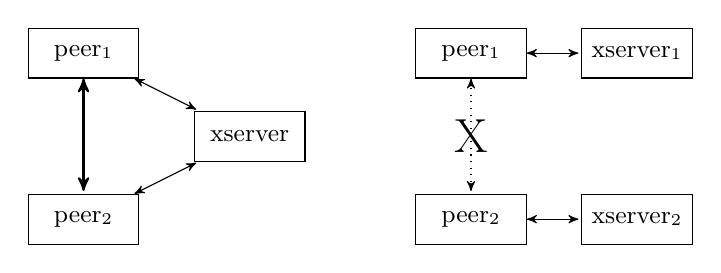
\begin{tikzpicture}[x=1pt,y=1pt,auto,start chain=going below]
                        \tikzstyle{every node}=[fill=none,rectangle,minimum height=0,draw,node distance=0,inner sep=0]
                        \tikzstyle{note}=[draw=none,opaque,fill=none]
                        \tikzstyle{xxx}=[minimum height=18,minimum width=40]
                        {
                            \node[xxx] (c1) at (-100, 30) {\small{peer$_1$}};
                            \node[xxx] (c2) at (-100, -30) {\small{peer$_2$}};
                            \node[xxx] (s1) at (-40, 0) {\small{xserver}};
                            \path[<->,>=stealth',shorten >=1,auto]
                                (c1) edge (s1)
                                (c2) edge (s1);
                            \path[<->,>=stealth',shorten >=1,auto,thick]
                                (c1) edge (c2);
                                
                            \node[xxx] (cx1) at (40, 30) {\small{peer$_1$}};
                            \node[xxx] (cx2) at (40, -30) {\small{peer$_2$}};
                            \node[xxx] (sx1) at (100, 30) {\small{xserver$_1$}};
                            \node[xxx] (sx2) at (100, -30) {\small{xserver$_2$}};
                            \path[<->,>=stealth',shorten >=1,auto]
                                (cx1) edge (sx1)
                                (cx2) edge (sx2);
                            \path[<->,>=stealth',shorten >=1,auto]
                                (cx1) edge[dotted] (cx2);
                            \draw let \p1=(cx1) in (\x1,\y1)
                                node[note] at (\x1,0) {\LARGE{X}};
                        }
                    \end{tikzpicture}
                }
                \end{figure}
                \end{small}
        }
        \only<3> {
            \item RPC应用场景
                \begin{itemize}
                    \item 视频内弹幕等
                    \item 游戏内状态、动作等等
                \end{itemize}
                \vskip1em
                \begin{small}
                \begin{figure}[h]
                \centering
                \scalebox{0.65}{
                    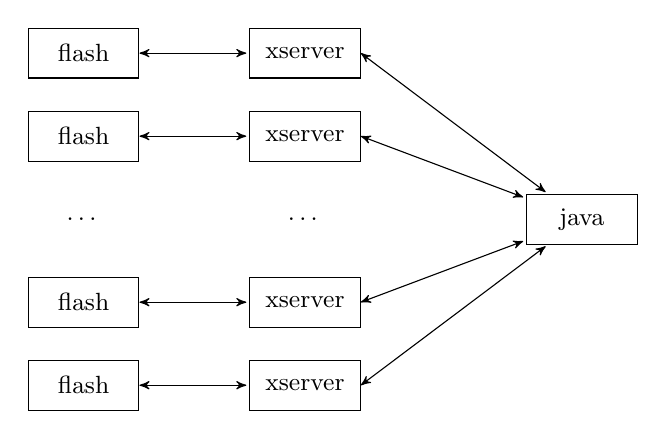
\begin{tikzpicture}[x=1pt,y=1pt,auto,start chain=going below]
                        \tikzstyle{every node}=[fill=none,rectangle,minimum height=0,draw,node distance=0,inner sep=0]
                        \tikzstyle{note}=[draw=none,opaque,fill=none]
                        \tikzstyle{xxx}=[minimum height=18,minimum width=40]
                        {
                            \node[xxx] (java) at (180, 0) {\small{java}};
                            
                            \newcount\dist
                            \foreach \number in {-2,-1,1,2} {
                                \dist=\number
                                \multiply\dist by 30
                                \node[xxx] (c\number) at (0, \dist) {\small{flash}};
                                \node[xxx] (s\number) at (80, \dist) {\small{xserver}};
                                \path[<->,>=stealth',shorten >=1,auto]
                                    (c\number) edge (s\number)
                                    (s\number.east) edge (java);
                            }
                            \node[note] at (0, 0) {\small{\ldots}};
                            \node[note] at (80, 0) {\small{\ldots}};
                        }
                    \end{tikzpicture}
                }
                \end{figure}
                \end{small}
        }
    \end{itemize}
\end{frame}

\begin{frame}[t]{为什么重构}
    \begin{itemize}
        \item 项目需求:需要深入了解RTMFP协议
        \item 可靠性差:
            \begin{itemize}
                \item 可攻击漏洞导致程序crash
                \item 内存泄漏或者BUG导致吃光CPU、内存等资源
                \item 程序僵死:服务无响应
            \end{itemize}
        \item 性能差:单线程易过载
            \begin{itemize}
                \item P2P过程2--3w连接数
                \item 100人/秒进入速度
            \end{itemize}
        \item 不易维护、不易监控、不宜调试等等
    \end{itemize}
\end{frame}

\begin{frame}[t]{xserver}
    \begin{itemize}
        \item 多线程:设计目标是P2P 20--30w并发连接无压力
            \begin{itemize}
                \item 实际情况:
                    \begin{itemize}
                        \item 27w连接;1200CPU(MAX=1600)
                        \item 单核250+人/秒的进入速度
                    \end{itemize}
            \end{itemize}
        \item 可靠性
        \item 可读性
            \begin{itemize}
                \item 尽保留P2P/RPC的最小实现
                \item 数据结构的提炼
                \item xserver = 50+文件/7k+行代码
            \end{itemize}
    \end{itemize}
\end{frame}

\section{建立连接}

\begin{frame}[t]{基本数据包}
    \begin{itemize}
        \item <1-> 基于UDP通信,单个数据包大小不超过1个MTU
        \item <1-> 数据内容通过AES128加密
            \begin{itemize}
                \item <1-> 对称加密算法:密钥同时用于加密、解密过程
                \item <1-> flash与xserver协商生成一对密钥分别用于上下行加密
                    \only<1> {
                        \vskip1em
                        \begin{small}
                        \begin{figure}[h]
                        \centering
                        \scalebox{0.95}{
                            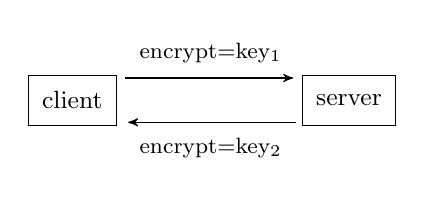
\begin{tikzpicture}[x=1pt,y=1pt,auto,start chain=going below]
                                \tikzstyle{every node}=[fill=none,rectangle,minimum height=18,draw,node distance=0,inner sep=5]
                                \tikzstyle{note}=[draw=none,opaque,fill=none]
                                \tikzstyle{hide}=[note,minimum width=0]
                                {

                                    \node (client) at (0, 0) {\small{client}};
                                    \node (server) at (100, 0) {\small{server}};
                                    \node[hide] (c1) at (14, 8) {};
                                    \node[hide] (c2) at (14, -8) {};
                                    \node[hide] (s1) at (86, 8) {};
                                    \node[hide] (s2) at (86, -8) {};
                                    \path[->,>=stealth',shorten >=1,auto]
                                        (c1) edge node[note,above] {\footnotesize{encrypt=key$_1$}} (s1)
                                        (s2) edge node[note,below] {\footnotesize{encrypt=key$_2$}} (c2);
                                }
                            \end{tikzpicture}
                        }
                        \end{figure}
                        \end{small}
                    }
                \item <2-> 两端分别维护数据结构保存密钥:数据包中记录解密id
                    \only<2> {
                        \begin{small}
                        \begin{figure}[h]
                        \centering
                        \scalebox{0.65}{
                            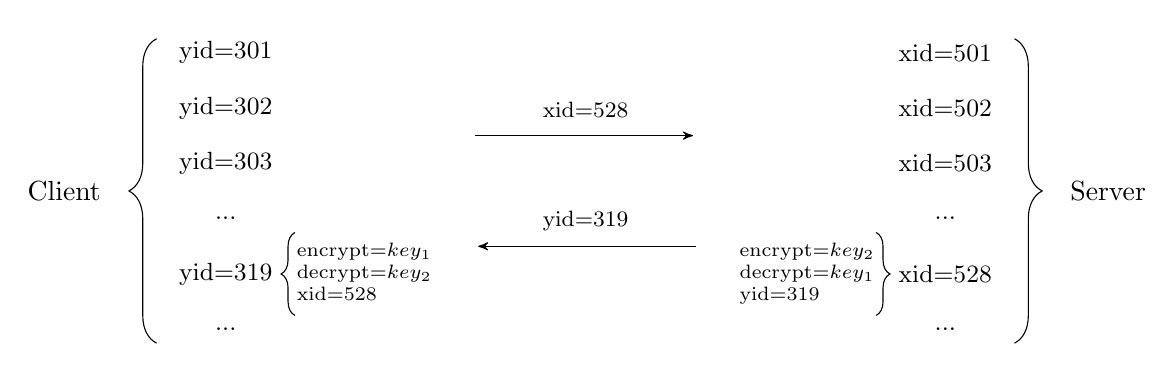
\begin{tikzpicture}[x=1pt,y=1pt,auto,start chain=going below]
                                \tikzstyle{every node}=[fill=none,rectangle,minimum height=18,draw,node distance=0,inner sep=0]
                                \tikzstyle{note}=[draw=none,opaque,fill=none]
                                \tikzstyle{hide}=[note,minimum width=0]
                                \tikzstyle{state}=[fill=white,circle,inner sep=0,minimum height=9]
                                {

                                    \node[note] (y0) at (-130, +50) {\small{yid=301}};
                                    \node[note,node distance=20] (y1) [below of=y0] {\small{yid=302}};
                                    \node[note,node distance=20] (y2) [below of=y1] {\small{yid=303}};
                                    \node[note,node distance=20] (y3) [below of=y2] {\small{...}};
                                    \node[note,node distance=20] (y4) [below of=y3] {\small{yid=319}};
                                    \node[note,node distance=20] (y5) [below of=y4] {\small{...}};

                                    \node[note,node distance=50] [right of=y4] {\scriptsize{\makecell[l]{encrypt=$key_1$\\decrypt=$key_2$\\xid=528}}};

                                    \node[note] (x0) at (130, +50) {\small{xid=501}};
                                    \node[note,node distance=20] (x1) [below of=x0] {\small{xid=502}};
                                    \node[note,node distance=20] (x2) [below of=x1] {\small{xid=503}};
                                    \node[note,node distance=20] (x3) [below of=x2] {\small{...}};
                                    \node[note,node distance=20] (x4) [below of=x3] {\small{xid=528}};
                                    \node[note,node distance=20] (x5) [below of=x4] {\small{...}};

                                    \node[note,node distance=50] [left of=x4] {\scriptsize{\makecell[l]{encrypt=$key_2$\\decrypt=$key_1$\\yid=319}}};

                                    \draw[decorate,decoration={brace,amplitude=10}]
		                                (-155,-55) -- (-155,55) node[hide,midway,xshift=-20] {Client};

                                    \draw[decorate,decoration={brace,amplitude=5}]
		                                (-105,-45) -- (-105,-15) node[hide,midway] {};

                                    \draw[decorate,decoration={brace,amplitude=10}]
		                                (155,55) -- (155,-55) node[hide,midway,xshift=20] {Server};

                                    \draw[decorate,decoration={brace,amplitude=5}]
		                                (105,-15) -- (105,-45) node[hide,midway] {};

                                    \node[hide] (a0) at (-40, 20) {};
                                    \node[hide] (a1) at (40, 20) {};

                                    \node[hide] (b0) at (-40, -20) {};
                                    \node[hide] (b1) at (40, -20) {};

                                    \path[->,>=stealth',shorten >=1,auto]
                                        (a0) edge node[note,above] {\footnotesize{xid=528}} (a1)
                                        (b1) edge node[note,above] {\footnotesize{yid=319}} (b0);
                                }
                            \end{tikzpicture}
                        }
                        \end{figure}
                        \end{small}
                    }
                \item <3-> 握手过程使用 id=0 以及默认密钥``Adobe Systems 02''
            \end{itemize}
    \end{itemize}
\end{frame}

\begin{frame}[t]{共享密钥生成}
    \begin{itemize}
        \only<1> {
            \item 通过非对称加密DH算法生成共享key
                \begin{small}
                \begin{figure}[h]
                \centering
                \scalebox{0.65}{
                    \begin{tikzpicture}[x=1pt,y=1pt,auto,start chain=going below]
                        \tikzstyle{every node}=[fill=none,rectangle,minimum height=18,draw,node distance=0,inner sep=0]
                        \tikzstyle{note}=[draw=none,opaque,fill=white]
                        \tikzstyle{hide}=[note,minimum width=0]
                        \tikzstyle{state}=[fill=white,circle,inner sep=0,minimum height=9]
                        {

                            \node[note] (text) at (-70, 0) {\small{已知 $g,p$}};
                            \node[note] (labels) at (0, +50) {Server};
                            \node[note] (labelc) at (0, -50) {Client};

                            \draw let \p1=(labelc.east) in (\x1,\y1)
                                node[hide,anchor=north west] {}
                                    [->] (\x1+10,\y1) -- +(340,0);

                            \draw let \p1=(labels.east) in (\x1,\y1)
                                node[hide,anchor=north west] {}
                                    [->] (\x1+10,\y1) -- +(340,0);

                            \node[state,node distance=80] (s1) [right of=labels] {};
                            \node[state,node distance=100] (s2) [right of=s1] {};

                            \node[state,node distance=80] (c1) [right of=labelc] {};
                            \node[state,node distance=100] (c2) [right of=c1] {};

                            \node[note,node distance=15] [above of=s1] {\footnotesize{$x_a=g^a \mod p$}};
                            \node[note,node distance=15] [below of=c1] {\footnotesize{$x_b=g^b \mod p$}};

                            \node[note,node distance=15] [above of=s2] {\footnotesize{$k_a=x_b^a \mod p$}};
                            \node[note,node distance=15] [below of=c2] {\footnotesize{$k_b=x_a^b \mod p$}};

                            \path[->,>=stealth',shorten >=1,auto]
                                (text) edge node[hide] {\footnotesize{$b=gen()$}} (labelc)
                                (text) edge node[hide] {\footnotesize{$a=gen()$}} (labels);

                            \path[->,>=stealth',shorten >=1,auto,dashed,thick]
                                (s1) edge (c2)
                                (c1) edge (s2);

                            \node[note,node distance=32] [below right of=s1] {\small{send $x_a$}};
                            \node[note,node distance=32] [above right of=c1] {\small{send $x_b$}};
                    }
                    \end{tikzpicture}
                }
                \end{figure}
                \end{small}
        }
        \only<2> {
            \item 两端各生成一个随机串并交换
                \begin{small}
                \begin{figure}[h]
                \centering
                \scalebox{0.65}{
                    \begin{tikzpicture}[x=1pt,y=1pt,auto,start chain=going below]
                        \tikzstyle{every node}=[fill=none,rectangle,minimum height=18,draw,node distance=0,inner sep=0]
                        \tikzstyle{note}=[draw=none,opaque,fill=white]
                        \tikzstyle{hide}=[note,minimum width=0]
                        \tikzstyle{state}=[fill=white,circle,inner sep=0,minimum height=9]
                        {

                            \node[note] (text) at (-70, 0) {\small{已知 $g,p$}};
                            \node[note] (labels) at (0, +50) {Server};
                            \node[note] (labelc) at (0, -50) {Client};

                            \draw let \p1=(labelc.east) in (\x1,\y1)
                                node[hide,anchor=north west] {}
                                    [->] (\x1+10,\y1) -- +(340,0);

                            \draw let \p1=(labels.east) in (\x1,\y1)
                                node[hide,anchor=north west] {}
                                    [->] (\x1+10,\y1) -- +(340,0);

                            \node[state,node distance=80] (s1) [right of=labels] {};
                            \node[state,node distance=100] (s2) [right of=s1] {};
                            \node[state,node distance=120] (s3) [right of=s2] {};

                            \node[state,node distance=80] (c1) [right of=labelc] {};
                            \node[state,node distance=100] (c2) [right of=c1] {};
                            \node[state,node distance=120] (c3) [right of=c2] {};

                            \node[note,node distance=15] [above of=s1] {\footnotesize{$x_a=g^a \mod p$}};
                            \node[note,node distance=15] [below of=c1] {\footnotesize{$x_b=g^b \mod p$}};

                            \node[note,node distance=15] [above of=s2] {\footnotesize{$k_a=x_b^a \mod p$}};
                            \node[note,node distance=15] [below of=c2] {\footnotesize{$k_b=x_a^b \mod p$}};

                            \path[->,>=stealth',shorten >=1,auto]
                                (text) edge node[hide] {\footnotesize{$b=gen()$}} (labelc)
                                (text) edge node[hide] {\footnotesize{$a=gen()$}} (labels);

                            \path[->,>=stealth',shorten >=1,auto,dashed,thick]
                                (s1) edge (c2)
                                (c1) edge (s2)
                                (s2) edge (c3)
                                (c2) edge (s3);

                            \node[note,node distance=32] [below right of=s1] {\small{send $x_a$}};
                            \node[note,node distance=32] [above right of=c1] {\small{send $x_b$}};

                            \node[note,node distance=32] [below right of=s2] {\small{send $\lambda_1$}};
                            \node[note,node distance=32] [above right of=c2] {\small{send $\lambda_2$}};
                    }
                    \end{tikzpicture}
                }
                \end{figure}
                \end{small}

        }
        \only<3> {
            \item 两端分别用共享key对随机串进行hash的到一组共享密钥
                \begin{small}
                \begin{figure}[h]
                \centering
                \scalebox{0.65}{
                    \begin{tikzpicture}[x=1pt,y=1pt,auto,start chain=going below]
                        \tikzstyle{every node}=[fill=none,rectangle,minimum height=18,draw,node distance=0,inner sep=0]
                        \tikzstyle{note}=[draw=none,opaque,fill=white]
                        \tikzstyle{hide}=[note,minimum width=0]
                        \tikzstyle{state}=[fill=white,circle,inner sep=0,minimum height=9]
                        {

                            \node[note] (text) at (-70, 0) {\small{已知 $g,p$}};
                            \node[note] (labels) at (0, +50) {Server};
                            \node[note] (labelc) at (0, -50) {Client};

                            \draw let \p1=(labelc.east) in (\x1,\y1)
                                node[hide,anchor=north west] {}
                                    [->] (\x1+10,\y1) -- +(340,0);

                            \draw let \p1=(labels.east) in (\x1,\y1)
                                node[hide,anchor=north west] {}
                                    [->] (\x1+10,\y1) -- +(340,0);

                            \node[state,node distance=80] (s1) [right of=labels] {};
                            \node[state,node distance=100] (s2) [right of=s1] {};
                            \node[state,node distance=120] (s3) [right of=s2] {};

                            \node[state,node distance=80] (c1) [right of=labelc] {};
                            \node[state,node distance=100] (c2) [right of=c1] {};
                            \node[state,node distance=120] (c3) [right of=c2] {};

                            \node[note,node distance=15] [above of=s1] {\footnotesize{$x_a=g^a \mod p$}};
                            \node[note,node distance=15] [below of=c1] {\footnotesize{$x_b=g^b \mod p$}};

                            \node[note,node distance=15] [above of=s2] {\footnotesize{$k_a=x_b^a \mod p$}};
                            \node[note,node distance=15] [below of=c2] {\footnotesize{$k_b=x_a^b \mod p$}};

                            \node[note,node distance=25] [above of=s3] {\footnotesize\makecell[c]{$encrypt=hmac(k_a, \lambda_2,\lambda_1)$\\$decrypt=hmac(k_a, \lambda_1,\lambda_2)$}};
                            \node[note,node distance=25] [below of=c3] {\footnotesize\makecell[c]{$encrypt=hmac(k_b, \lambda_1,\lambda_2)$\\$decrypt=hmac(k_b, \lambda_2,\lambda_1)$}};

                            \path[->,>=stealth',shorten >=1,auto]
                                (text) edge node[hide] {\footnotesize{$b=gen()$}} (labelc)
                                (text) edge node[hide] {\footnotesize{$a=gen()$}} (labels);

                            \path[->,>=stealth',shorten >=1,auto,dashed,thick]
                                (s1) edge (c2)
                                (c1) edge (s2)
                                (s2) edge (c3)
                                (c2) edge (s3);

                            \node[note,node distance=32] [below right of=s1] {\small{send $x_a$}};
                            \node[note,node distance=32] [above right of=c1] {\small{send $x_b$}};

                            \node[note,node distance=32] [below right of=s2] {\small{send $\lambda_1$}};
                            \node[note,node distance=32] [above right of=c2] {\small{send $\lambda_2$}};
                    }
                    \end{tikzpicture}
                }
                \end{figure}
                \end{small}
        }
    \end{itemize}
\end{frame}

\begin{frame}[t]{握手过程}
    \begin{itemize}
        \item <1-> 探测对方并对应用进行验证
            \only<1> {
                \begin{small}
                \begin{figure}[h]
                \centering
                \scalebox{0.65}{
                    \begin{tikzpicture}[x=1pt,y=1pt,auto,start chain=going below]
                        \tikzstyle{every node}=[fill=none,rectangle,minimum height=18,draw,node distance=0,inner sep=0]
                        \tikzstyle{note}=[draw=none,opaque,fill=white]
                        \tikzstyle{hide}=[note,minimum width=0]
                        \tikzstyle{state}=[fill=white,circle,inner sep=0,minimum height=9]
                        {

                            \node[note] (labels) at (0, +50) {Server};
                            \node[note] (labelc) at (0, -50) {Client};

                            \draw let \p1=(labelc.east) in (\x1,\y1)
                                node[hide,anchor=north west] {}
                                    [->] (\x1+10,\y1) -- +(340,0);

                            \draw let \p1=(labels.east) in (\x1,\y1)
                                node[hide,anchor=north west] {}
                                    [->] (\x1+10,\y1) -- +(340,0);

                            \node[state,node distance=60] (c1) [right of=labelc] {};
                            \node[state,node distance=120] (c2) [right of=c1] {};
                            \node[state,node distance=120] (s1) [right of=labels] {};

                            \path[->,>=stealth',shorten >=1,auto,thick]
                                (c1) edge (s1)
                                (s1) edge (c2);

                            \node[note,node distance=42] [above right of=c1] {\footnotesize{msg=$\{app\}$}};
                            \node[note,node distance=42] [below right of=s1] {\footnotesize{msg=$\{cookie\}$}};
                        }
                    \end{tikzpicture}
                }
                \end{figure}
                \end{small}

            }
        \item <2-> 进行DH算法生成密钥
            \only<2> {
                \begin{small}
                \begin{figure}[h]
                \centering
                \scalebox{0.65}{
                    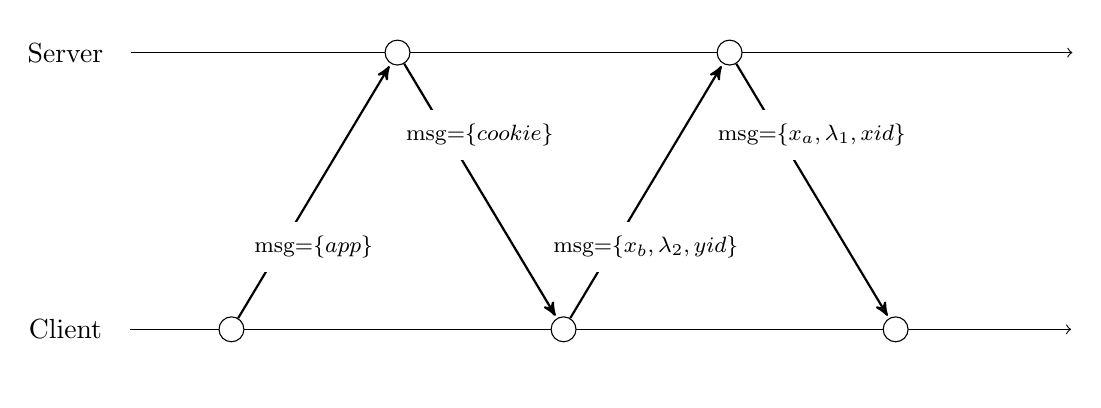
\begin{tikzpicture}[x=1pt,y=1pt,auto,start chain=going below]
                        \tikzstyle{every node}=[fill=none,rectangle,minimum height=18,draw,node distance=0,inner sep=0]
                        \tikzstyle{note}=[draw=none,opaque,fill=white]
                        \tikzstyle{hide}=[note,minimum width=0]
                        \tikzstyle{state}=[fill=white,circle,inner sep=0,minimum height=9]
                        {

                            \node[note] (labels) at (0, +50) {Server};
                            \node[note] (labelc) at (0, -50) {Client};

                            \draw let \p1=(labelc.east) in (\x1,\y1)
                                node[hide,anchor=north west] {}
                                    [->] (\x1+10,\y1) -- +(340,0);

                            \draw let \p1=(labels.east) in (\x1,\y1)
                                node[hide,anchor=north west] {}
                                    [->] (\x1+10,\y1) -- +(340,0);

                            \node[state,node distance=60] (c1) [right of=labelc] {};
                            \node[state,node distance=120] (c2) [right of=c1] {};
                            \node[state,node distance=120] (c3) [right of=c2] {};
                            \node[state,node distance=120] (s1) [right of=labels] {};
                            \node[state,node distance=120] (s2) [right of=s1] {};

                            \path[->,>=stealth',shorten >=1,auto,thick]
                                (c1) edge (s1)
                                (s1) edge (c2)
                                (c2) edge (s2)
                                (s2) edge (c3);

                            \node[note,node distance=42] [above right of=c1] {\footnotesize{msg=$\{app\}$}};
                            \node[note,node distance=42] [below right of=s1] {\footnotesize{msg=$\{cookie\}$}};
                            \node[note,node distance=42] [above right of=c2] {\footnotesize{msg=$\{x_b,\lambda_2,yid\}$}};
                            \node[note,node distance=42] [below right of=s2] {\footnotesize{msg=$\{x_a,\lambda_1,xid\}$}};
                        }
                    \end{tikzpicture}
                }
                \end{figure}
                \end{small}
            }
    \end{itemize}
\end{frame}

\section{数据流}

\begin{frame}[t]{多层结构}
    \begin{itemize}
        \only<1,2> {
            \item 应用层:产生数据,并对数据进行封装
            \only<2> {
                \vskip1em
                \begin{small}
                \begin{figure}[h]
                \centering
                \scalebox{0.65}{
                    \begin{tikzpicture}[x=1pt,y=1pt,auto]
                        \tikzstyle{every node}=[fill=none,rectangle,minimum height=18,draw,node distance=0,inner sep=0]
                        \tikzstyle{note}=[draw=none,opaque,fill=none]
                        \tikzstyle{hide}=[note,minimum width=0]
                        \tikzstyle{data} = [draw=black,minimum width=20, minimum height=20, node distance=20,fill=white]
                        \tikzstyle{data0} = [data,fill=gray!25]
                        \tikzstyle{data1} = [data,fill=gray!55]
                        {
                            \newcount\dist
                            \foreach \number in {0,1,2,3,4,5,8,9,10} {
                                \dist=\number
                                \multiply\dist by 20
                                \node[data0] (a\number) at (\dist,0) {};
                            }
                            \node[note] at (130, 0) {\small{\ldots}};
                            \node[note,node distance=35] [left of=a0] {data};

                            \foreach \number in {0,1,4,5} {
                                \dist=\number
                                \multiply\dist by 20
                                \node[data,fill=white] (b\number) at (\dist,-50) {};
                            }
                            \foreach \number in {6,7,8,9,10,11,14,15,16} {
                                \dist=\number
                                \multiply\dist by 20
                                \node[data0] (b\number) at (\dist,-50) {};
                            }
                            \node[note] at (50, -50) {\small{\ldots}};
                            \node[note] at (250, -50) {\small{\ldots}};
                            \node[note,node distance=35] [left of=b0] {object};

                            \path[->,>=stealth',shorten >=1,shorten <=1,auto]
                                (a0.south) edge (b6.north)
                                (a10.south) edge (b16.north);

                            \draw[decorate,decoration={brace,amplitude=3}]
			                    (110,-65) -- (-10,-65) node[hide,midway] {\footnotesize{amf header:回调函数类型、名称等等}};
                        }
                    \end{tikzpicture}
                }
                \end{figure}
                \end{small}
            }
        }
        \only<1,3> {
            \item 数据流:缓存应用层数据,维护传输可靠性
            \only<3> {
                \begin{itemize}
                    \item 对数据进行切片并分配序号
                    \item 切片大:切片个数少,减少传输成本
                    \item 切片小:UDP包数量少,组装灵活
                \end{itemize}
                \vskip1em
                \begin{small}
                \begin{figure}[h]
                \centering
                \scalebox{0.55}{
                    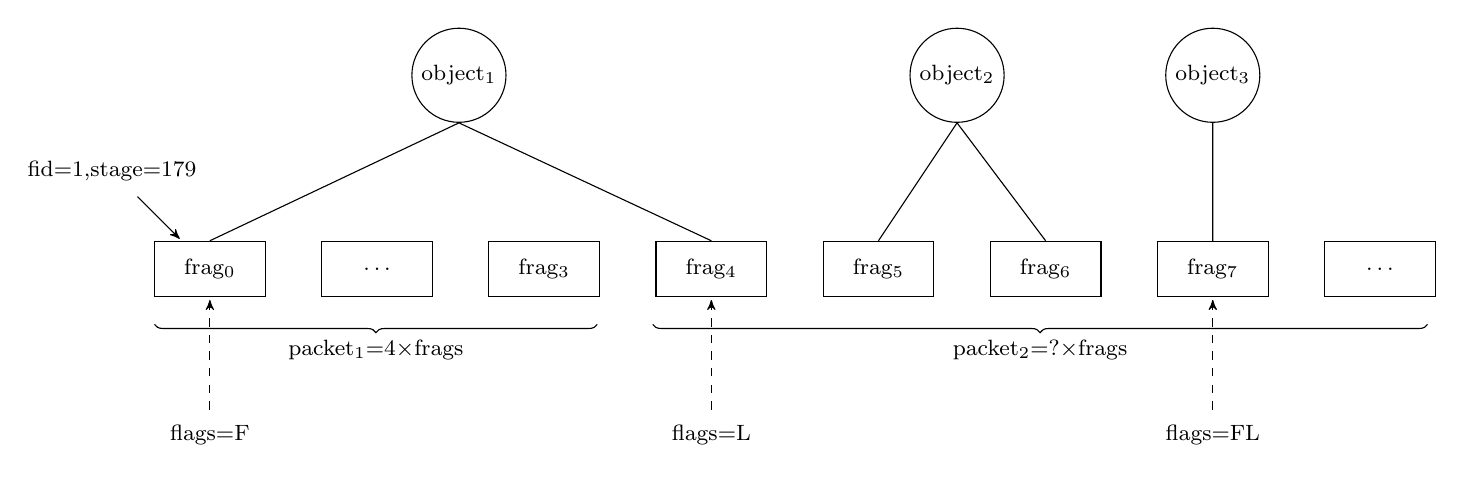
\begin{tikzpicture}[x=1pt,y=1pt,auto,start chain=1 going right]]
                        \tikzstyle{every node}=[fill=none,rectangle,minimum height=18,draw,node distance=0,inner sep=0]
                        \tikzstyle{note}=[draw=none,opaque,fill=none]
                        \tikzstyle{hide}=[note,minimum width=0]
                        \tikzstyle{object}=[fill=white,circle,inner sep=0,minimum height=34]
                        \tikzstyle{fragment} = [draw=black,minimum width=40, minimum height=20, node distance=20,fill=white]
                        {
                            \node[fragment,on chain=1] (a0) {\footnotesize{frag$_0$}};
                            \node[fragment,on chain=1] (a1) {\footnotesize{$\dots$}};
                            \node[fragment,on chain=1] (a2) {\footnotesize{frag$_3$}};
                            \node[fragment,on chain=1] (a3) {\footnotesize{frag$_4$}};
                            \node[fragment,on chain=1] (a4) {\footnotesize{frag$_5$}};
                            \node[fragment,on chain=1] (a5) {\footnotesize{frag$_6$}};
                            \node[fragment,on chain=1] (a6) {\footnotesize{frag$_7$}};
                            \node[fragment,on chain=1] (a7) {\footnotesize{$\dots$}};
                            
                            \node[note,node distance=50] (ax) [above left of=a0] {\footnotesize{fid=1,stage=179}};
                            
                            \node[note,node distance=60] (a0b) [below of=a0] {\footnotesize{flags=F}};
                            \node[note,node distance=60] (a3b) [below of=a3] {\footnotesize{flags=L}};
                            \node[note,node distance=60] (a6b) [below of=a6] {\footnotesize{flags=FL}};
                            
                            \path[->,>=stealth',shorten >=1pt,auto]
                                (ax) edge (a0)
                                (a0b) edge[dashed] (a0)
                                (a3b) edge[dashed] (a3)
                                (a6b) edge[dashed] (a6);

                            \node[object] (b0) at (90, 70) {\footnotesize{object$_1$}};
                            \node[object] (b1) at (270, 70) {\footnotesize{object$_2$}};
                            \draw let \p1=(a6.north) in (\x1,\y1)
                                node[object] (b2) at (\x1, 70) {\footnotesize{object$_3$}};

                            \path[draw]
                                (b0.south) -- (a0.north)
                                (b0.south) -- (a3.north)
                                (b1.south) -- (a4.north)
                                (b1.south) -- (a5.north)
                                (b2.south) -- (a6.north);

                            \draw[decorate,decoration={brace,amplitude=3}]
			                    (140,-20) -- (-20,-20) node[hide,midway] {\footnotesize{packet$_1$=4$\times$frags}};
                            \draw[decorate,decoration={brace,amplitude=3}]
			                    (440,-20) -- (160,-20) node[hide,midway] {\footnotesize{packet$_2$=?$\times$frags}};
                        }
                    \end{tikzpicture}
                }
                \end{figure}
                \end{small}
            }
        }
        \only<1,4> {
            \item 数据片:数据发送最小单元
            \only<4> {
                \begin{small}
                \begin{figure}[h]
                \centering
                \scalebox{0.65}{
                    \begin{tikzpicture}[x=1pt,y=1pt,auto]
                        \tikzstyle{every node}=[fill=none,rectangle,minimum height=18,draw,node distance=0,inner sep=0]
                        \tikzstyle{note}=[draw=none,opaque,fill=none]
                        \tikzstyle{hide}=[note,minimum width=0]
                        \tikzstyle{data} = [draw=black,minimum width=20, minimum height=20, node distance=20,fill=white]
                        \tikzstyle{data0} = [data,fill=gray!15]
                        \tikzstyle{data1} = [data,fill=gray!85]
                        \tikzstyle{data2} = [data,postaction={pattern=north east lines}]
                        \tikzstyle{data3} = [data,fill=gray!55]
                        {
                            \newcount\dist
                            \foreach \number in {0} {
                                \dist=\number
                                \multiply\dist by 20
                                \node[data0] (a\number) at (\dist,-50) {\scriptsize{0x10}};
                            }
                            \foreach \number in {1,2} {
                                \dist=\number
                                \multiply\dist by 20
                                \node[data1] (a\number) at (\dist,-50) {};
                            }
                            \foreach \number in {3,4,7,8} {
                                \dist=\number
                                \multiply\dist by 20
                                \node[data2] (a\number) at (\dist,-50) {};
                            }
                            \node[note] at (110, -50) {\small{\ldots}};

                            \draw[decorate,decoration={brace,amplitude=3}]
	                            (50,-35) -- (170,-35) node[hide,midway] {\footnotesize{内容共size字节}};

                            \draw[decorate,decoration={brace,amplitude=3}]
	                            (50,-65) -- (10,-65) node[hide,midway] {\footnotesize{size}};
                            \draw[decorate,decoration={brace,amplitude=3}]
	                            (10,-65) -- (-10,-65) node[hide,midway] {\footnotesize{code}};
                            \node[note,node distance=45] [left of=a0] {\small{0x10数据片}};

                            \foreach \number in {1} {
                                \dist=\number
                                \multiply\dist by 20
                                \node[data3,minimum width=20] (b\number) at (20+\dist,-100) {\scriptsize{flags}};
                            }
                            \foreach \number in {3} {
                                \dist=\number
                                \multiply\dist by 20
                                \node[data0,minimum width=40] (b\number) at (10+\dist,-100) {\scriptsize{fid}};
                            }
                            \foreach \number in {6} {
                                \dist=\number
                                \multiply\dist by 20
                                \node[data3,minimum width=100] (b\number) at (20+\dist,-100) {\scriptsize{headers}};
                            }
                            \foreach \number in {10} {
                                \dist=\number
                                \multiply\dist by 20
                                \node[data0,minimum width=60] (b\number) at (20+\dist,-100) {\scriptsize{$\dots$}};
                            }
                            \path[draw]
                                (a3.south) -- (b1.north west)
                                (a8.south) -- (b10.north east);
                        }
                        {
                            \newcount\dist
                            \foreach \number in {0} {
                                \dist=\number
                                \multiply\dist by 20
                                \node[data0] (c\number) at (\dist,-150) {\scriptsize{0x11}};
                            }
                            \foreach \number in {1,2} {
                                \dist=\number
                                \multiply\dist by 20
                                \node[data1] (c\number) at (\dist,-150) {};
                            }
                            \foreach \number in {3,4,7,8} {
                                \dist=\number
                                \multiply\dist by 20
                                \node[data2] (c\number) at (\dist,-150) {};
                            }
                            \node[note] at (110, -150) {\small{\ldots}};
                            
                            \draw[decorate,decoration={brace,amplitude=3}]
			                    (50,-135) -- (170,-135) node[hide,midway] {\footnotesize{内容共size字节}};

                            \draw[decorate,decoration={brace,amplitude=3}]
			                    (50,-165) -- (10,-165) node[hide,midway] {\footnotesize{size}};
                            \draw[decorate,decoration={brace,amplitude=3}]
			                    (10,-165) -- (-10,-165) node[hide,midway] {\footnotesize{code}};
                            \node[note,node distance=45] [left of=c0] {\small{0x11数据片}};

                            \foreach \number in {1} {
                                \dist=\number
                                \multiply\dist by 20
                                \node[data3,minimum width=20] (d\number) at (20+\dist,-200) {\scriptsize{flags}};
                            }
                            \foreach \number in {3} {
                                \dist=\number
                                \multiply\dist by 20
                                \node[data0,minimum width=60] (d\number) at (20+\dist,-200) {\scriptsize{$\dots$}};
                            }
                            \path[draw]
                                (c3.south) -- (d1.north west)
                                (c8.south) -- (d3.north east);

                            \foreach \number in {0,4} {
                                \dist=\number
                                \multiply\dist by 40
                                \node[data0,minimum width=40] (e\number) at (\dist,-250) {\scriptsize{0x10}};
                            }
                            \foreach \number in {1,2,3,5,6} {
                                \dist=\number
                                \multiply\dist by 40
                                \node[data3,minimum width=40] (e\number) at (\dist,-250) {\scriptsize{0x11}};
                            }
                            \draw[decorate,decoration={brace,amplitude=3}]
			                    (20,-265) -- (-20,-265) node[hide,midway] {\footnotesize{fid=1,stage=127}};
                            \draw[decorate,decoration={brace,amplitude=3}]
			                    (180,-265) -- (140,-265) node[hide,midway] {\footnotesize{fid=1,stage=135}};
                            \draw[decorate,decoration={brace,amplitude=3}]
			                    (20,-235) -- (140,-235) node[hide,midway] {\footnotesize{stage=128,129,130}};
                            \draw[decorate,decoration={brace,amplitude=3}]
			                    (180,-235) -- (260,-235) node[hide,midway] {\footnotesize{stage=136,137}};

                            \node[note,node distance=30] [below of=e2] {\small{多数据片拼接}};
                        }
                    \end{tikzpicture}
                }
                \end{figure}
                \end{small}
            }
        }
        \only<5> {
            \item 数据包:包含一个或者多个数据片,并加密
                \begin{small}
                \begin{figure}[h]
                \centering
                \scalebox{0.65}{
                    \begin{tikzpicture}[x=1pt,y=1pt,auto]
                        \tikzstyle{every node}=[fill=none,rectangle,minimum height=18,draw,node distance=0,inner sep=0]
                        \tikzstyle{note}=[draw=none,opaque,fill=none]
                        \tikzstyle{hide}=[note,minimum width=0]
                        \tikzstyle{data} = [draw=black,minimum width=20, minimum height=20, node distance=20,fill=white]
                        \tikzstyle{data0} = [data,fill=gray!15]
                        \tikzstyle{data1} = [data,fill=gray!85]
                        \tikzstyle{data2} = [data,postaction={pattern=north east lines}]
                        {
                            \newcount\dist
                            \foreach \number in {-3} {
                                \dist=\number
                                \multiply\dist by 20
                                \node[data0] (b\number) at (\dist,-50) {};
                            }
                            \foreach \number in {-2,-1} {
                                \dist=\number
                                \multiply\dist by 20
                                \node[data1] (b\number) at (\dist,-50) {};
                            }
                            \foreach \number in {0,9} {
                                \dist=\number
                                \multiply\dist by 20
                                \node[data0] (b\number) at (\dist,-50) {};
                            }
                            \foreach \number in {1,2,10,11} {
                                \dist=\number
                                \multiply\dist by 20
                                \node[data1] (b\number) at (\dist,-50) {};
                            }
                            \foreach \number in {3,4,7,8,12,13} {
                                \dist=\number
                                \multiply\dist by 20
                                \node[data2] (b\number) at (\dist,-50) {};
                            }
                            \node[note] at (110, -50) {\small{\ldots}};
                            \node[note] at (290, -50) {\small{\ldots \ldots}};
                            \node[note,node distance=35] [left of=b-3] {数据包};

                            \draw[decorate,decoration={brace,amplitude=3}]
			                    (50,-35) -- (170,-35) node[hide,midway] {\footnotesize{内容共size字节}};

                            \draw[decorate,decoration={brace,amplitude=3}]
			                    (-50,-35) -- (-10,-35) node[hide,midway] {\footnotesize{time}};
                            \draw[decorate,decoration={brace,amplitude=3}]
			                    (-50,-65) -- (-70,-65) node[hide,midway] {\footnotesize{mark}};

                            \draw[decorate,decoration={brace,amplitude=3}]
			                    (50,-65) -- (10,-65) node[hide,midway] {\footnotesize{size}};
                            \draw[decorate,decoration={brace,amplitude=3}]
			                    (10,-65) -- (-10,-65) node[hide,midway] {\footnotesize{code}};

                            \draw[decorate,decoration={brace,amplitude=3}]
			                    (190,-65) -- (170,-65) node[hide,midway] {\footnotesize{code}};
                            \draw[decorate,decoration={brace,amplitude=3}]
			                    (230,-65) -- (190,-65) node[hide,midway] {\footnotesize{size}};

                            \draw[decorate,decoration={brace,amplitude=3}]
			                    (310,-85) -- (-10,-85) node[hide,midway] {\footnotesize{多个数据片}};
                        }
                    \end{tikzpicture}
                }
                \end{figure}
                \end{small}
                \begin{itemize}
                    \item 控制片:心跳请求与响应、关闭连接请求、数据包ack等等
                    \item 流数据:0x10 数据片、0x11 数据片
                \end{itemize}
        }
        \only<1> {
            \vskip1em
            \begin{small}
            \begin{figure}[h]
            \centering
            \scalebox{0.65}{
                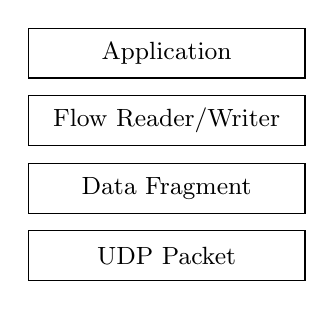
\begin{tikzpicture}[x=1pt,y=1pt,auto,start chain=1 going above]
                    \tikzstyle{every node}=[fill=none,rectangle,minimum height=18,minimum width=100,draw,node distance=6,inner sep=4]
                    {
                        \node[on chain=1] {\small{UDP Packet}};
                        \node[on chain=1] {\small{Data Fragment}};
                        \node[on chain=1] {\small{Flow Reader/Writer}};
                        \node[on chain=1] {\small{Application}};
                    }
                \end{tikzpicture}
            }
            \end{figure}
            \end{small}
        }
    \end{itemize}
\end{frame}

\begin{frame}[t]{UDP数据包生成}
    \begin{itemize}
        \item <1-> 拷贝数据包内容到缓冲区并填充0xff补全
            \only<1> {
                \begin{small}
                \begin{figure}[h]
                \centering
                \scalebox{0.65}{
                    \begin{tikzpicture}[x=1pt,y=1pt,auto]
                        \tikzstyle{every node}=[fill=none,rectangle,minimum height=18,draw,node distance=0,inner sep=0]
                        \tikzstyle{note}=[draw=none,opaque,fill=none]
                        \tikzstyle{hide}=[note,minimum width=0]
                        \tikzstyle{data} = [draw=black,minimum width=20, minimum height=20, node distance=20,fill=white]
                        \tikzstyle{data0} = [data,fill=gray!25]
                        \tikzstyle{data1} = [data,fill=gray!55]
                        {
                            \newcount\dist
                            \foreach \number in {0,1,2,3,4,5,8,9,10} {
                                \dist=\number
                                \multiply\dist by 20
                                \node[data0] (a\number) at (\dist,0) {};
                            }
                            \node[note] at (130, 0) {\small{\ldots}};
                            \node[note,node distance=35] [left of=a0] {数据包};

                            \foreach \number in {0,1,2,3,4,5} {
                                \dist=\number
                                \multiply\dist by 20
                                \node[data,fill=white] (b\number) at (\dist,-50) {};
                            }
                            \foreach \number in {6,7,8,9,10,11,14,15,16} {
                                \dist=\number
                                \multiply\dist by 20
                                \node[data0] (b\number) at (\dist,-50) {};
                            }
                            \foreach \number in {17,18,19} {
                                \dist=\number
                                \multiply\dist by 20
                                \node[data1] (b\number) at (\dist,-50) {\scriptsize{0xff}};
                            }
                            \node[note] at (250, -50) {\small{\ldots}};
                            \node[note,node distance=35] [left of=b0] {缓冲区};

                            \path[->,>=stealth',shorten >=1,shorten <=1,auto]
                                (a0.south) edge (b6.north)
                                (a10.south) edge (b16.north);

                            \draw[decorate,decoration={brace,amplitude=3}]
			                    (390,-65) -- (70,-65) node[hide,midway] {\footnotesize{AES128 16字节对齐:不足则用0xff补齐}};
                        }
                    \end{tikzpicture}
                }
                \end{figure}
                \end{small}
            }
        \item <2-> 生成数据校验和并使用加密密钥加密
            \only<2> {
                \begin{small}
                \begin{figure}[h]
                \centering
                \scalebox{0.65}{
                    \begin{tikzpicture}[x=1pt,y=1pt,auto]
                        \tikzstyle{every node}=[fill=none,rectangle,minimum height=18,draw,node distance=0,inner sep=0]
                        \tikzstyle{note}=[draw=none,opaque,fill=none]
                        \tikzstyle{hide}=[note,minimum width=0]
                        \tikzstyle{data} = [draw=black,minimum width=20, minimum height=20, node distance=20,fill=white]
                        \tikzstyle{data0} = [data,fill=gray!25]
                        \tikzstyle{data1} = [data,fill=gray!55]
                        \tikzstyle{data2} = [data,postaction={pattern=crosshatch dots}]
                        \tikzstyle{data3} = [data,fill=gray!10,postaction={pattern=north east lines,pattern color=black!70}]
                        {
                            \newcount\dist
                            \foreach \number in {0,1,2,3} {
                                \dist=\number
                                \multiply\dist by 20
                                \node[data,fill=white] (b\number) at (\dist,-50) {};
                            }
                            \foreach \number in {4,5} {
                                \dist=\number
                                \multiply\dist by 20
                                \node[data2] (b\number) at (\dist,-50) {};
                            }
                            \foreach \number in {6,7,8,9,10,11,14,15,16} {
                                \dist=\number
                                \multiply\dist by 20
                                \node[data0] (b\number) at (\dist,-50) {};
                            }
                            \foreach \number in {17,18,19} {
                                \dist=\number
                                \multiply\dist by 20
                                \node[data1] (b\number) at (\dist,-50) {\scriptsize{0xff}};
                            }
                            \node[note] at (250, -50) {\small{\ldots}};
                            \node[note,node distance=35] [left of=b0] {缓冲区};

                            \draw[decorate,decoration={brace,amplitude=3}]
			                    (110,-35) -- (390,-35) node[hide,midway] {\footnotesize{计算校验和checksum}};

                            \draw[decorate,decoration={brace,amplitude=3}]
			                    (110,-65) -- (70,-65) node[hide,midway] {\footnotesize{checksum}};

                            \foreach \number in {0,1,2,3} {
                                \dist=\number
                                \multiply\dist by 20
                                \node[data,fill=white] (c\number) at (\dist,-110) {};
                            }
                            \foreach \number in {4,5,6,7,8,9,10,11,14,15,16,17,18,19} {
                                \dist=\number
                                \multiply\dist by 20
                                \node[data3] (c\number) at (\dist,-110) {};
                            }
                            \node[note] at (250, -110) {\small{\ldots}};
                            \node[note,node distance=35] [left of=c0] {缓冲区};

                            \draw[decorate,decoration={brace,amplitude=3}]
			                    (390,-125) -- (70,-125) node[hide,midway] {\footnotesize{AES128对数据加密}};
                        }
                    \end{tikzpicture}
                }
                \end{figure}
                \end{small}
            }
        \item <3-> 写入对端id信息
            \only<3> {
                \begin{small}
                \begin{figure}[h]
                \centering
                \scalebox{0.65}{
                    \begin{tikzpicture}[x=1pt,y=1pt,auto]
                        \tikzstyle{every node}=[fill=none,rectangle,minimum height=18,draw,node distance=0,inner sep=0]
                        \tikzstyle{note}=[draw=none,opaque,fill=none]
                        \tikzstyle{hide}=[note,minimum width=0]
                        \tikzstyle{data} = [draw=black,minimum width=20, minimum height=20, node distance=20,fill=white]
                        \tikzstyle{data0} = [data,postaction={pattern=crosshatch dots}]
                        \tikzstyle{data1} = [data,postaction={pattern=north east lines,pattern color=black!70}]
                        {
                            \newcount\dist
                            \foreach \number in {0,1,2,3} {
                                \dist=\number
                                \multiply\dist by 20
                                \node[data0] (b\number) at (\dist,-50) {};
                            }
                            \foreach \number in {4,5,6,7,8,9,10,11,14,15,16,17,18,19} {
                                \dist=\number
                                \multiply\dist by 20
                                \node[data1] (b\number) at (\dist,-50) {};
                            }
                            \node[note] at (250, -50) {\small{\ldots}};
                            \node[note,node distance=35] [left of=b0] {缓冲区};

                            \draw[decorate,decoration={brace,amplitude=3}]
			                    (150,-65) -- (70,-65) node[hide,midway] {\footnotesize{$p_1$}};

                            \draw[decorate,decoration={brace,amplitude=3}]
			                    (230,-65) -- (150,-65) node[hide,midway] {\footnotesize{$p_2$}};

                            \draw[decorate,decoration={brace,amplitude=3}]
			                    (70,-65) -- (-10,-65) node[hide,midway] {\footnotesize{$p_0=yid \oplus p_1 \oplus p_2$}};
                        }
                    \end{tikzpicture}
                }
                \end{figure}
                \end{small}
            }
    \end{itemize}
\end{frame}

\begin{frame}[t]{Reliable通信过程}
    \begin{itemize}
        \only<1> {
            \item 写入数据 obj=\{m$_{23}$,m$_{24}$,m$_{25}$\}
            \begin{small}
            \begin{figure}[h]
            \centering
            \scalebox{0.65}{
                \begin{tikzpicture}[x=1pt,y=1pt,auto]
                    \tikzstyle{every node}=[fill=none,rectangle,minimum height=18,draw,node distance=0,inner sep=0]
                    \tikzstyle{note}=[draw=none,above,opaque,fill=none]
                    \tikzstyle{hide}=[note,minimum width=0]
                    \tikzstyle{state}=[fill=white,circle,inner sep=0,minimum height=9]
                    {
                        \node[note] (labelc) at (0, 0) {Client};
                        \node[note] (labels) at (100, 0) {Server};

                        \draw let \p1=(labelc.south) in (\x1,\y1)
                            node[hide,anchor=north west] {}
                                [->] (\x1,\y1-3) -- +(0,-220);

                        \draw let \p1=(labels.south) in (\x1,\y1)
                            node[hide,anchor=north west] {}
                                [->] (\x1,\y1-3) -- +(0,-220);
                                
                        \node[state,node distance=25] (s1) [below of=labels] {};
                        \node[state,node distance=25] (s2) [below of=s1] {};
                        \node[state,node distance=25] (s3) [below of=s2] {};
                        \node[state,node distance=50] (c1) [below of=labelc] {};
                        \node[state,node distance=25] (c2) [below of=c1] {};
                        \node[state,node distance=25] (c3) [below of=c2] {};

                        \node[note,node distance=60,text width=100] [left of=c1] {};
                        \node[note,node distance=60,text width=100] [right of=s1] {};
                        
                        \node[note,node distance=60,text width=100] [right of=s1] {\footnotesize{cache=\{23,24,25\}}};

                        \path[above,every node/.style={font=\sffamily\tiny}]
                            (s1) -- node[sloped] {msg=23} (c1)
                            (s2) -- node[sloped] {msg=24} (c2)
                            (s3) -- node[sloped] {msg=25} (c3);

                        \path[->,>=stealth',shorten >=1pt,auto]
                            (s1) edge[dashed] (c1)
                            (s2) edge[dashed] (c2)
                            (s3) edge[dashed] (c3);
                    }
                \end{tikzpicture}
            }
            \end{figure}
            \end{small}
        }
        \only<2> {
            \item 主动对最后一个数据包进行丢包重传
            \begin{small}
            \begin{figure}[h]
            \centering
            \scalebox{0.65}{
                \begin{tikzpicture}[x=1pt,y=1pt,auto]
                    \tikzstyle{every node}=[fill=none,rectangle,minimum height=18,draw,node distance=0,inner sep=0]
                    \tikzstyle{note}=[draw=none,above,opaque,fill=none]
                    \tikzstyle{hide}=[note,minimum width=0]
                    \tikzstyle{state}=[fill=white,circle,inner sep=0,minimum height=9]
                    {
                        \node[note] (labelc) at (0, 0) {Client};
                        \node[note] (labels) at (100, 0) {Server};
                        \node[note] at (50, -20) {\rotatebox{90}{\footnotesize{\ldots\ldots}}};

                        \draw let \p1=(labelc.south) in (\x1,\y1)
                            node[hide,anchor=north west] {}
                                [->] (\x1,\y1-3) -- +(0,-220);

                        \draw let \p1=(labels.south) in (\x1,\y1)
                            node[hide,anchor=north west] {}
                                [->] (\x1,\y1-3) -- +(0,-220);
                                
                        \node[state,node distance=35] (s1) [below of=labels] {};
                        \node[state,node distance=25] (s2) [below of=s1] {};
                        \node[state,node distance=25] (s3) [below of=s2] {};
                        \node[state,node distance=60] (c1) [below of=labelc] {};
                        \node[state,node distance=25] (c2) [below of=c1] {};
                        \node[state,node distance=25] (c3) [below of=c2] {};
                        
                        \node[note,node distance=60,text width=100] [left of=c1] {};
                        \node[note,node distance=60,text width=100] [right of=s1] {};
                        
                        \node[note,node distance=60,text width=100] [right of=s1] {\footnotesize{cache=\{23,24,25\}}};
                        \node[note,node distance=60,text width=100] [left of=c3] {\hfill\footnotesize{buffer=\{25\}}};
                        
                        \path[above,every node/.style={font=\sffamily\tiny}]
                            (s1) -- node[sloped] {msg=25} (c1)
                            (s2) -- node[sloped] {msg=25} (c2)
                            (s3) -- node[sloped] {msg=25} (c3);

                        \path[->,>=stealth',shorten >=1pt,auto]
                            (s1) edge[dashed] (c1)
                            (s2) edge[dashed] (c2)
                            (s3) edge (c3);
                    }
                \end{tikzpicture}
            }
            \end{figure}
            \end{small}
        }
        \only<3> {
            \item 收到消息立即返回ack
            \begin{small}
            \begin{figure}[h]
            \centering
            \scalebox{0.65}{
                \begin{tikzpicture}[x=1pt,y=1pt,auto]
                    \tikzstyle{every node}=[fill=none,rectangle,minimum height=18,draw,node distance=0,inner sep=0]
                    \tikzstyle{note}=[draw=none,above,opaque,fill=none]
                    \tikzstyle{hide}=[note,minimum width=0]
                    \tikzstyle{state}=[fill=white,circle,inner sep=0,minimum height=9]
                    {
                        \node[note] (labelc) at (0, 0) {Client};
                        \node[note] (labels) at (100, 0) {Server};
                        \node[note] at (50, -20) {\rotatebox{90}{\footnotesize{\ldots\ldots}}};

                        \draw let \p1=(labelc.south) in (\x1,\y1)
                            node[hide,anchor=north west] {}
                                [->] (\x1,\y1-3) -- +(0,-220);

                        \draw let \p1=(labels.south) in (\x1,\y1)
                            node[hide,anchor=north west] {}
                                [->] (\x1,\y1-3) -- +(0,-220);
                                
                        \node[state,node distance=35] (s1) [below of=labels] {};
                        \node[state,node distance=25] (s2) [below of=s1] {};
                        \node[state,node distance=25] (s3) [below of=s2] {};
                        \node[state,node distance=50] (s4) [below of=s3] {};
                        \node[state,node distance=60] (c1) [below of=labelc] {};
                        \node[state,node distance=25] (c2) [below of=c1] {};
                        \node[state,node distance=25] (c3) [below of=c2] {};
                        
                        \node[note,node distance=60,text width=100] [left of=c1] {};
                        \node[note,node distance=60,text width=100] [right of=s1] {};
                        
                        \node[note,node distance=60,text width=100] [right of=s1] {\footnotesize{cache=\{23,24,25\}}};
                        \node[note,node distance=60,text width=100] [left of=c3] {\hfill\footnotesize{buffer=\{25\}}};
                        \node[note,node distance=60,text width=100] [right of=s4] {\footnotesize{cache=\{23,24\}}};
                        
                        \path[above,every node/.style={font=\sffamily\tiny}]
                            (s1) -- node[sloped] {msg=25} (c1)
                            (s2) -- node[sloped] {msg=25} (c2)
                            (s3) -- node[sloped] {msg=25} (c3)
                            (c3) -- node[sloped] {ack=25,miss=23,24} (s4);

                        \path[->,>=stealth',shorten >=1pt,auto]
                            (s1) edge[dashed] (c1)
                            (s2) edge[dashed] (c2)
                            (s3) edge (c3)
                            (c3) edge (s4);
                    }
                \end{tikzpicture}
            }
            \end{figure}
            \end{small}
        }
        \only<4> {
            \item ack驱动丢包重传
            \begin{small}
            \begin{figure}[h]
            \centering
            \scalebox{0.65}{
                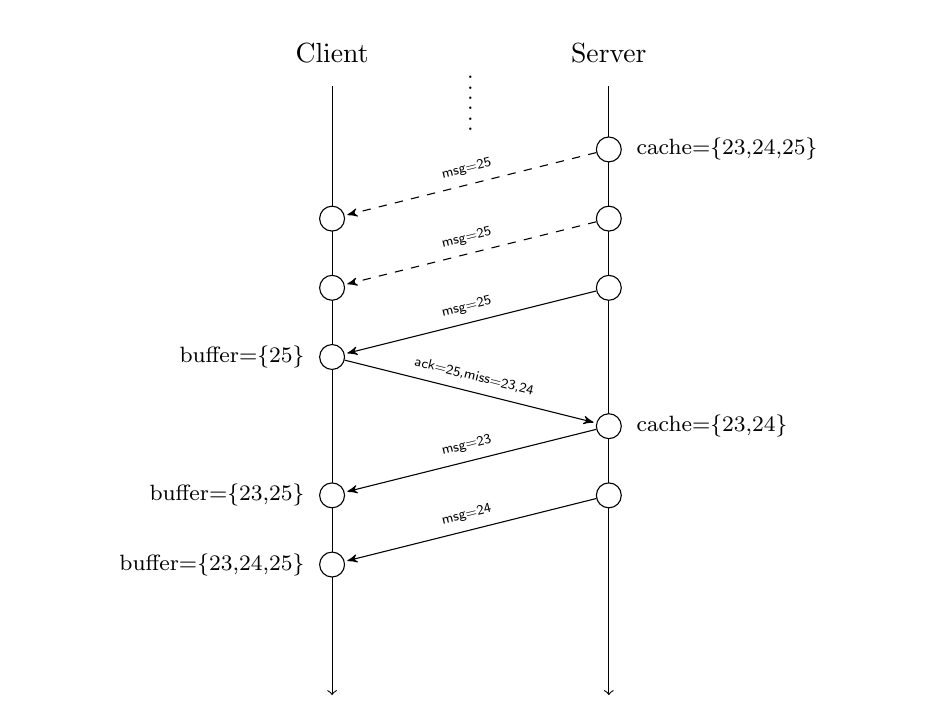
\begin{tikzpicture}[x=1pt,y=1pt,auto]
                    \tikzstyle{every node}=[fill=none,rectangle,minimum height=18,draw,node distance=0,inner sep=0]
                    \tikzstyle{note}=[draw=none,above,opaque,fill=none]
                    \tikzstyle{hide}=[note,minimum width=0]
                    \tikzstyle{state}=[fill=white,circle,inner sep=0,minimum height=9]
                    {
                        \node[note] (labelc) at (0, 0) {Client};
                        \node[note] (labels) at (100, 0) {Server};
                        \node[note] at (50, -20) {\rotatebox{90}{\footnotesize{\ldots\ldots}}};

                        \draw let \p1=(labelc.south) in (\x1,\y1)
                            node[hide,anchor=north west] {}
                                [->] (\x1,\y1-3) -- +(0,-220);

                        \draw let \p1=(labels.south) in (\x1,\y1)
                            node[hide,anchor=north west] {}
                                [->] (\x1,\y1-3) -- +(0,-220);
                                
                        \node[state,node distance=35] (s1) [below of=labels] {};
                        \node[state,node distance=25] (s2) [below of=s1] {};
                        \node[state,node distance=25] (s3) [below of=s2] {};
                        \node[state,node distance=50] (s4) [below of=s3] {};
                        \node[state,node distance=25] (s5) [below of=s4] {};
                        \node[state,node distance=60] (c1) [below of=labelc] {};
                        \node[state,node distance=25] (c2) [below of=c1] {};
                        \node[state,node distance=25] (c3) [below of=c2] {};
                        \node[state,node distance=50] (c4) [below of=c3] {};
                        \node[state,node distance=25] (c5) [below of=c4] {};
                        
                        \node[note,node distance=60,text width=100] [left of=c1] {};
                        \node[note,node distance=60,text width=100] [right of=s1] {};
                        
                        \node[note,node distance=60,text width=100] [right of=s1] {\footnotesize{cache=\{23,24,25\}}};
                        \node[note,node distance=60,text width=100] [right of=s4] {\footnotesize{cache=\{23,24\}}};
                        \node[note,node distance=60,text width=100] [left of=c3] {\hfill\footnotesize{buffer=\{25\}}};
                        \node[note,node distance=60,text width=100] [left of=c4] {\hfill\footnotesize{buffer=\{23,25\}}};
                        \node[note,node distance=60,text width=100] [left of=c5] {\hfill\footnotesize{buffer=\{23,24,25\}}};
                        
                        \path[above,every node/.style={font=\sffamily\tiny}]
                            (s1) -- node[sloped] {msg=25} (c1)
                            (s2) -- node[sloped] {msg=25} (c2)
                            (s3) -- node[sloped] {msg=25} (c3)
                            (s4) -- node[sloped] {msg=23} (c4)
                            (s5) -- node[sloped] {msg=24} (c5)
                            (c3) -- node[sloped] {ack=25,miss=23,24} (s4);

                        \path[->,>=stealth',shorten >=1pt,auto]
                            (s1) edge[dashed] (c1)
                            (s2) edge[dashed] (c2)
                            (s3) edge (c3)
                            (c3) edge (s4)
                            (s4) edge (c4)
                            (s5) edge (c5);
                    }
                \end{tikzpicture}
            }
            \end{figure}
            \end{small}
        }
        \only<5> {
            \item 收到数据包deliver消息并返回ack
            \begin{small}
            \begin{figure}[h]
            \centering
            \scalebox{0.65}{
                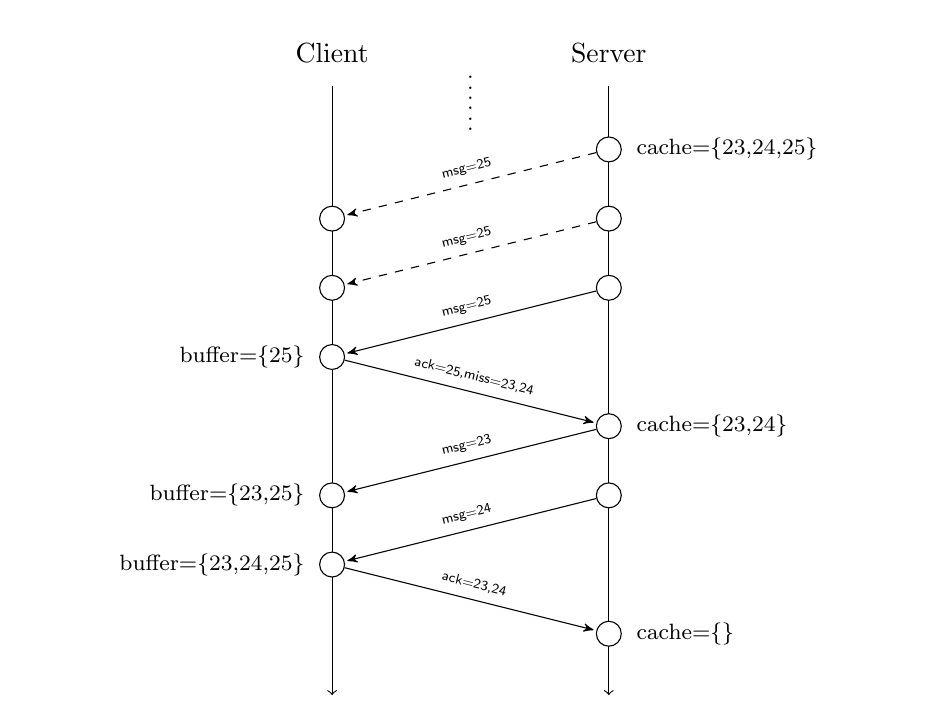
\begin{tikzpicture}[x=1pt,y=1pt,auto]
                    \tikzstyle{every node}=[fill=none,rectangle,minimum height=18,draw,node distance=0,inner sep=0]
                    \tikzstyle{note}=[draw=none,above,opaque,fill=none]
                    \tikzstyle{hide}=[note,minimum width=0]
                    \tikzstyle{state}=[fill=white,circle,inner sep=0,minimum height=9]
                    {
                        \node[note] (labelc) at (0, 0) {Client};
                        \node[note] (labels) at (100, 0) {Server};
                        \node[note] at (50, -20) {\rotatebox{90}{\footnotesize{\ldots\ldots}}};

                        \draw let \p1=(labelc.south) in (\x1,\y1)
                            node[hide,anchor=north west] {}
                                [->] (\x1,\y1-3) -- +(0,-220);

                        \draw let \p1=(labels.south) in (\x1,\y1)
                            node[hide,anchor=north west] {}
                                [->] (\x1,\y1-3) -- +(0,-220);
                                
                        \node[state,node distance=35] (s1) [below of=labels] {};
                        \node[state,node distance=25] (s2) [below of=s1] {};
                        \node[state,node distance=25] (s3) [below of=s2] {};
                        \node[state,node distance=50] (s4) [below of=s3] {};
                        \node[state,node distance=25] (s5) [below of=s4] {};
                        \node[state,node distance=50] (s6) [below of=s5] {};
                        \node[state,node distance=60] (c1) [below of=labelc] {};
                        \node[state,node distance=25] (c2) [below of=c1] {};
                        \node[state,node distance=25] (c3) [below of=c2] {};
                        \node[state,node distance=50] (c4) [below of=c3] {};
                        \node[state,node distance=25] (c5) [below of=c4] {};
                        
                        \node[note,node distance=60,text width=100] [left of=c1] {};
                        \node[note,node distance=60,text width=100] [right of=s1] {};
                        
                        \node[note,node distance=60,text width=100] [right of=s1] {\footnotesize{cache=\{23,24,25\}}};
                        \node[note,node distance=60,text width=100] [right of=s4] {\footnotesize{cache=\{23,24\}}};
                        \node[note,node distance=60,text width=100] [right of=s6] {\footnotesize{cache=\{\}}};
                        \node[note,node distance=60,text width=100] [left of=c3] {\hfill\footnotesize{buffer=\{25\}}};
                        \node[note,node distance=60,text width=100] [left of=c4] {\hfill\footnotesize{buffer=\{23,25\}}};
                        \node[note,node distance=60,text width=100] [left of=c5] {\hfill\footnotesize{buffer=\{23,24,25\}}};
                        
                        \path[above,every node/.style={font=\sffamily\tiny}]
                            (s1) -- node[sloped] {msg=25} (c1)
                            (s2) -- node[sloped] {msg=25} (c2)
                            (s3) -- node[sloped] {msg=25} (c3)
                            (s4) -- node[sloped] {msg=23} (c4)
                            (s5) -- node[sloped] {msg=24} (c5)
                            (c3) -- node[sloped] {ack=25,miss=23,24} (s4)
                            (c5) -- node[sloped] {ack=23,24} (s6);

                        \path[->,>=stealth',shorten >=1pt,auto]
                            (s1) edge[dashed] (c1)
                            (s2) edge[dashed] (c2)
                            (s3) edge (c3)
                            (c3) edge (s4)
                            (s4) edge (c4)
                            (s5) edge (c5)
                            (c5) edge (s6);
                    }
                \end{tikzpicture}
            }
            \end{figure}
            \end{small}
        }
    \end{itemize}
\end{frame}

\begin{frame}[t]{Unreliable通信过程}
    \begin{itemize}
        \only<1,2> {
            \item 协议中,Sender在发送数据时,还返回从Receiver发来的ack的ack$^*$!!
            \begin{small}
            \begin{center}
                ack=$[0, $ack$^*]\cup[s_0,s_1]\cup[s_2,s_3]\cup\dots\cup[s_{2n},s_{2_n+1}]$\\其中 $s_{2i+1}+1<s_{2i+2}, i\geq0$
            \end{center}
            \end{small}
            \begin{itemize}
                \item ack$^*$表示Receiver收到的最大连续stage序号
                \only<2> {
                    \item 实践中发现:ack$^*$对于Receiver还表示stage$\leq$ack$^*$的消息Sender都不再缓存!!
                }
            \end{itemize}
        }
        \only<3> {
            \item 写入数据 obj$_1$=\{m$_{23}$,m$_{24}$\}
            \begin{small}
            \begin{figure}[h]
            \centering
            \scalebox{0.65}{
                \begin{tikzpicture}[x=1pt,y=1pt,auto]
                    \tikzstyle{every node}=[fill=none,rectangle,minimum height=18,draw,node distance=0,inner sep=0]
                    \tikzstyle{note}=[draw=none,above,opaque,fill=none]
                    \tikzstyle{hide}=[note,minimum width=0]
                    \tikzstyle{state}=[fill=white,circle,inner sep=0,minimum height=9]
                    {
                        \node[note] (labelc) at (0, 0) {Client};
                        \node[note] (labels) at (150, 0) {Server};

                        \draw let \p1=(labelc.south) in (\x1,\y1)
                            node[hide,anchor=north west] {}
                                [->] (\x1,\y1-3) -- +(0,-220);

                        \draw let \p1=(labels.south) in (\x1,\y1)
                            node[hide,anchor=north west] {}
                                [->] (\x1,\y1-3) -- +(0,-220);
                                
                        \node[state,node distance=35] (s1) [below of=labels] {};
                        \node[state,node distance=25] (s2) [below of=s1] {};
                        \node[state,node distance=60] (c1) [below of=labelc] {};
                        \node[state,node distance=25] (c2) [below of=c1] {};
                        
                        \node[note,node distance=80,text width=140] [left of=c1] {};
                        \node[note,node distance=80,text width=140] [right of=s1] {};
                        
                        \node[note,node distance=80,text width=140] (x) [right of=s1] {\footnotesize{cache=\{23,24\},ack$^*$=22}};
                        \node[note,node distance=20] [below of=x] {\footnotesize{cache=\{\},ack$^*$=24}};
                        
                        \node[note,node distance=80,text width=140] [left of=c1] {\hfill\footnotesize{buffer=\{23\}}};
                        \node[note,node distance=80,text width=140] [left of=c2] {\hfill\footnotesize{buffer=\{23\}}};
                        
                        \draw let \p1=(s1) in (\x1,\y1)
                            node[hide,anchor=north west] {}
                                [->] (\x1+20,\y1-8) -- +(18,-8);
                                
                        \path[above,every node/.style={font=\sffamily\tiny}]
                            (s1) -- node[sloped] {msg=23,ack$^*$=22} (c1)
                            (s2) -- node[sloped] {msg=24,ack$^*$=22} (c2);

                        \path[->,>=stealth',shorten >=1pt,auto]
                            (s1) edge (c1)
                            (s2) edge[dashed] (c2);
                    }
                \end{tikzpicture}
            }
            \end{figure}
            \end{small}
        }
        \only<4> {
            \item 写入数据 obj$_2$=\{m$_{25}$\}
            \begin{small}
            \begin{figure}[h]
            \centering
            \scalebox{0.65}{
                \begin{tikzpicture}[x=1pt,y=1pt,auto]
                    \tikzstyle{every node}=[fill=none,rectangle,minimum height=18,draw,node distance=0,inner sep=0]
                    \tikzstyle{note}=[draw=none,above,opaque,fill=none]
                    \tikzstyle{hide}=[note,minimum width=0]
                    \tikzstyle{state}=[fill=white,circle,inner sep=0,minimum height=9]
                    {
                        \node[note] (labelc) at (0, 0) {Client};
                        \node[note] (labels) at (150, 0) {Server};

                        \draw let \p1=(labelc.south) in (\x1,\y1)
                            node[hide,anchor=north west] {}
                                [->] (\x1,\y1-3) -- +(0,-220);

                        \draw let \p1=(labels.south) in (\x1,\y1)
                            node[hide,anchor=north west] {}
                                [->] (\x1,\y1-3) -- +(0,-220);
                                
                        \node[state,node distance=35] (s1) [below of=labels] {};
                        \node[state,node distance=25] (s2) [below of=s1] {};
                        \node[state,node distance=25] (s3) [below of=s2] {};
                        \node[state,node distance=50] (s4) [below of=s3] {};
                        \node[state,node distance=60] (c1) [below of=labelc] {};
                        \node[state,node distance=25] (c2) [below of=c1] {};
                        \node[state,node distance=25] (c3) [below of=c2] {};
                        
                        \node[note,node distance=80,text width=140] [left of=c1] {};
                        \node[note,node distance=80,text width=140] [right of=s1] {};
                        
                        \node[note,node distance=80,text width=140] (x) [right of=s3] {\footnotesize{cache=\{25\},ack$^*$=24}};
                        \node[note,node distance=20] [below of=x] {\footnotesize{cache=\{\},ack$^*$=25}};
                        
                        \node[note,node distance=80,text width=140] [right of=s4] {\footnotesize{cache=\{\},ack$^*$=25}};
                        \node[note,node distance=80,text width=140] [left of=c1] {\hfill\footnotesize{buffer=\{23\}}};
                        \node[note,node distance=80,text width=140] [left of=c2] {\hfill\footnotesize{buffer=\{23\}}};
                        \node[note,node distance=80,text width=140] [left of=c3] {\hfill\footnotesize{buffer=\{25\}}};
                        
                        \draw let \p1=(s3) in (\x1,\y1)
                            node[hide,anchor=north west] {}
                                [->] (\x1+20,\y1-8) -- +(18,-8);
                                
                        \path[above,every node/.style={font=\sffamily\tiny}]
                            (s1) -- node[sloped] {msg=23,ack$^*$=22} (c1)
                            (s2) -- node[sloped] {msg=24,ack$^*$=22} (c2)
                            (s3) -- node[sloped] {msg=25,ack$^*$=24} (c3)
                            (c3) -- node[sloped] {ack=25} (s4);

                        \path[->,>=stealth',shorten >=1pt,auto]
                            (s1) edge (c1)
                            (s2) edge[dashed] (c2)
                            (s3) edge (c3)
                            (c3) edge (s4);
                    }
                \end{tikzpicture}
            }
            \end{figure}
            \end{small}
        }
    \end{itemize}
\end{frame}

\section{P2P过程}

\begin{frame}[t]{P2P打洞}
    \begin{itemize}
        \only<1> {
            \item P$_1$发起与P$_2$的P2P过程
                \begin{itemize}
                    \item P$_1$将P$_2$.pid 发送给服务端
                    \item 服务端向两边返回对方的信息
                \end{itemize}
            \begin{small}
            \begin{figure}[h!]
            \centering
            \scalebox{0.65}{
                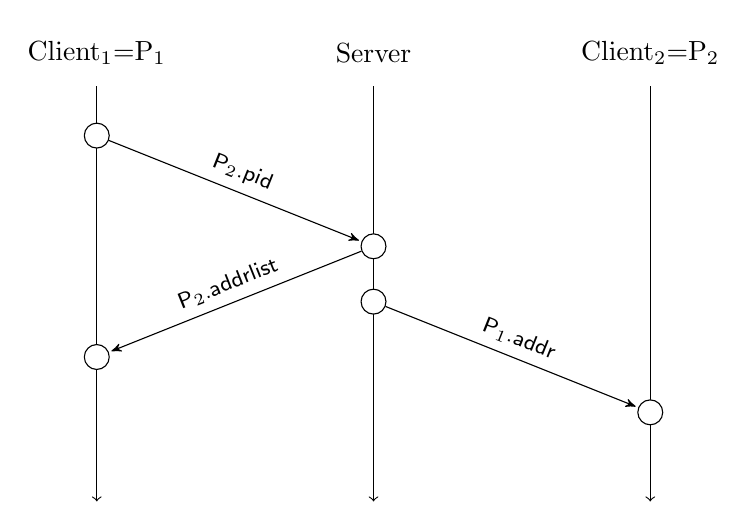
\begin{tikzpicture}[x=1pt,y=1pt,auto]
                    \tikzstyle{every node}=[fill=none,rectangle,minimum height=18,draw,node distance=0,inner sep=0]
                    \tikzstyle{note}=[draw=none,above,opaque,fill=none]
                    \tikzstyle{hide}=[note,minimum width=0]
                    \tikzstyle{state}=[fill=white,circle,inner sep=0,minimum height=9]
                    {
                        \node[note] (labelc1) at (-100, 0) {Client$_1$=P$_1$};
                        \node[note] (labels) at (0, 0) {Server};
                        \node[note] (labelc2) at (100, 0) {Client$_2$=P$_2$};

                        \draw let \p1=(labelc1.south) in (\x1,\y1)
                            node[hide,anchor=north west] {}
                                [->] (\x1,\y1-3) -- +(0,-150);

                        \draw let \p1=(labelc2.south) in (\x1,\y1)
                            node[hide,anchor=north west] {}
                                [->] (\x1,\y1-3) -- +(0,-150);

                        \draw let \p1=(labels.south) in (\x1,\y1)
                            node[hide,anchor=north west] {}
                                [->] (\x1,\y1-3) -- +(0,-150);

                        \node[state,node distance=30] (c1) [below of=labelc1] {};
                        \node[state,node distance=80] (c2) [below of=c1] {};
                        \node[state,node distance=70] (s1) [below of=labels] {};
                        \node[state,node distance=20] (s2) [below of=s1] {};
                        \node[state,node distance=130] (c3) [below of=labelc2] {};

                        \path[->,>=stealth',shorten >=1pt,auto]
                            (c1) edge (s1)
                            (s1) edge (c2)
                            (s2) edge (c3);
                        \path[above,every node/.style={font=\sffamily\footnotesize}]
                            (s1) -- node[sloped] {P$_2$.pid} (c1)
                            (s1) -- node[sloped] {P$_2$.addrlist} (c2)
                            (s2) -- node[sloped] {P$_1$.addr} (c3);
                    }
                \end{tikzpicture}
            }
            \end{figure}
            \end{small}
        }
        \only<2> {
            \item 双方打洞
                \begin{itemize}
                    \item P$_1$向获取到的P$_2$的所有地址发送request
                    \item P$_2$向获取到的P$_1$的地址发送response
                \end{itemize}
                            \begin{small}
            \begin{figure}[h!]
            \centering
            \scalebox{0.65}{
                \begin{tikzpicture}[x=1pt,y=1pt,auto]
                    \tikzstyle{every node}=[fill=none,rectangle,minimum height=18,draw,node distance=0,inner sep=5]
                    \tikzstyle{note}=[draw=none,above,opaque,fill=none]
                    \tikzstyle{hide}=[note,minimum width=0,minimum height=0,inner sep=0]
                    \tikzstyle{cc}=[fill=white,circle,inner sep=0,minimum height=9]
                    {
                        \node[draw] (labelc1) at (-100, 0) {Client$_1$=P$_1$};
                        \node[draw] (labelc2) at (100, 0) {Client$_2$=P$_2$};

                        \node[cc,minimum height=120,fill=none,dashed] at (-100, 0) {};
                        \node[cc,minimum height=120,fill=none,dashed] at (100, 0) {};
                        
                        \foreach \number in {-1,-2,1,2} {
                            \dist=\number
                            \multiply\dist by -30
                            \node[hide] (c\number) at (-10,\dist) {};
                        }
                        
                        \node[hide] (d) at (10,0) {};
                        
                        \path[->,>=stealth',shorten >=1pt,auto]
                            (labelc1) edge (c-1)
                            (labelc1) edge (c-2)
                            (labelc1) edge (c1)
                            (labelc1) edge (c2)
                            (labelc2) edge (d);
                            
                        \path[above,every node/.style={font=\sffamily\tiny}]
                            (labelc1) -- node[sloped] {P$_2$.addr[0]} (c-2)
                            (labelc1) -- node[sloped] {P$_2$.addr[1]} (c-1)
                            (labelc1) -- node[sloped] {P$_2$.addr[2]} (c1)
                            (labelc1) -- node[sloped] {P$_2$.addr[3]} (c2)
                            (labelc2) -- node[sloped] {P$_1$.addr} (d);
                    }
                \end{tikzpicture}
            }
            \end{figure}
            \end{small}
        }
    \end{itemize}
\end{frame}

\section{Go语言}

\begin{frame}[t]{为什么选择Go}
    \begin{itemize}
        \only<1> {
            \item 编译执行
                \begin{itemize}
                    \item 编译速度快 - C语言爱好者
                    \item 命令行开发、调试+linux工具链
                \end{itemize}
            \item 运行效率
                \begin{itemize}
                    \item c > go > c++
                    \item 代码质量影响大于语言选择
                \end{itemize}
            \item 开发效率
                \begin{itemize}
                    \item 自带内存gc
                    \item 保留但是弱化指针
                \end{itemize}
        }
        \only<2,3> {
            \item 语法简洁
                \begin{itemize}
                    \only<2> {
                        \item 简单的类声明、初始化:编译器做最少的事情
                            \only<2> {
                                \begin{itemize}
                                    \item c++ 的构造函数、析构函数、虚函数?
                                    \item java 的构造函数执行顺序?
                                \end{itemize}
                            }
                        \item 空 != null:减少错误和参数检查
                            \only<2> {
                                \begin{itemize}
                                    \item 空字符串 = ""
                                    \item 空数组 = []类型
                                \end{itemize}
                            }
                    }
                    \only<3> {
                        \item 内置切片 slice
                        \item 多函数返回值
                        \item 错误处理:error ? panic ?
                        \item defer 比 finally 更强大
                        \item 语法更灵活:闭包+函数类型
                    }
                \end{itemize}
        }
        \only<4> {
            \item routine 概念
                \begin{itemize}
                    \item 轻量级线程:fiber?
                \end{itemize}
            \item channel 概念
                \begin{itemize}
                    \item 管道?
                    \item 生产者+消费者 $\rightarrow$ 线程同步
                \end{itemize}
        }
    \end{itemize}
\end{frame}

\end{document}
